\section{Assurances}
    The term assurances was introduced in the previous section as the name by which feedback will be known in a human-AIA trust relationship. A more detailed definition and discussion is merited.

    \citet{McKnight2001-fa} alludes to this kind of feedback in an e-commerce relationship as `Web Vendor Interventions' and mentions some possible actions that might be used in that specific application. They go as far as making a diagram that indicates that these interventions could affect the `Trusting Beliefs', `Trusting Intentions', and `Trust-Related Behaviors' (see Figure \ref{fig:UserTrust}).
    
    The term is perhaps earliest used in the context of human-automation relationships by \citet{Sheridan1984-kx}. More recently, and formally, \citet{Lillard2016-yg} defined the term `assurances' as (modified to fit the AIA terminology):
    
    \begin{description}
        \item [Assurances:] The AIA's ability to affect the user's trust. As used here, the term is not intended to have a positive or negative connotation -- assurances can decrease trust.
    \end{description}

	\begin{figure}[htbp]
    	\centering
     	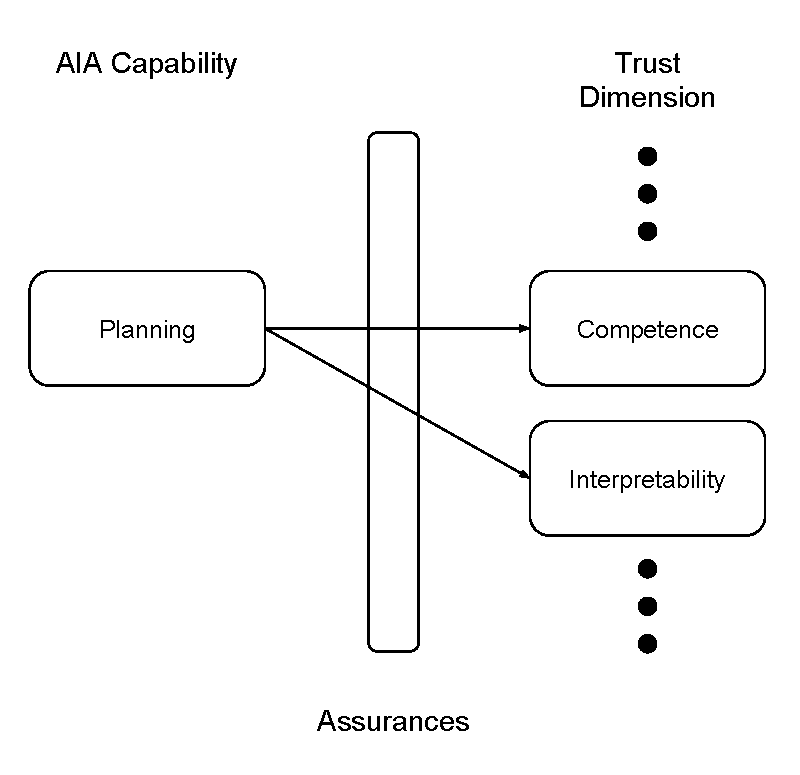
\includegraphics[width=0.4\textwidth]{Figures/Assurance_mapping.pdf}
    	\caption{Assurances act as a mapping between AIA capabilities and the components of User trust. Shown in this figure, An example of assurances that operate on planning algorithms and output something that is interpreted by the user, and will affect their trust.}
        \label{fig:assurance_mapping}
    \end{figure}
    
    

    Figure \ref{fig:Assurance_classes} shows the hierarchy of proposed assurance classes. The categories mirror those of the trust model proposed by \citet{McKnight2001-fa}, but with the emphasis on what an AIA has the ability to most readily influence (and consequently where most research is found). The colored boxes identify the different classes assurances. All classes are included here for completeness and generality. Although, due to practical limitations it might hypothetically be possible for an AIA to influence a persons general `Trusting stance' given enough time\footnote{One might imagine an AIA that specifically speaks to the human about the benefits or drawbacks about trusting even though there might not be evidence to do so, similar to the role a counselor might play}.

    Talk about the two classes of assurances: Unintentional and Intentional.

    \begin{description}
        \item [Unintentional:] Assurances that are not purposfully given by AI. Could be compared to non-verbal communication\ldots well not quite
        \begin{itemize}
            \item Such as success in completing the task (of course the autonomy wants to, but the outcome is independent).
            \item The way an autonomous vehicle looks when it is driving (something with weird driving habits for whatever reason might engender less trust). 
            \item 
        \end{itemize}
        \item [Intentional:] Assurances that are purposefully given by AI.
        \begin{itemize}
            \item Legible motion
            \item $R^2$
            \item Counter planning
            \item task similarity (to ideal task)
            \item etc.
        \end{itemize}
    \end{description}

    Each type of assurance can be given in unintentional or intentional ways. Perhaps they can be treated analogously to actions and words, specifically `actions speak louder than words' or `unintentional assurances speak louder than intentional ones'. The point is that actually doing something instead of just saying it will do a lot for bolstering trust. What is better saying: I can do this, or actually doing it?

    However, for the case of calibrating TRBs it is proposed that the classes should be constrained as shown in Figure \ref{fig:Assurance_classes}. An AI that is trying to calibrate the TRBs of a user (as opposed to just influencing them to its own benefit), should not actively try to convice the user that it should have faith in autonomy, or that it is benevolent, or that the institutional system should be trusted.

    Due to the nature of trust a single assurance might be targeted at influencing the competence dimension of trust, but it will likely also have affects on other dimensions. As an example an assurance aimed at influencing Predictability may also have an affect on the Probability of Depending.

    Besides being difficult to separate, each user is different. Thus no assurance will work identically when given to two separate users.

    \textbf{I am not sure how I want this argument to go, I want to highlight that it is theoretically possible to have some affect on each of these attributes, but that some are more practical. Two main things need to be considred 1) time-scale (how long will it take to make a noticeable change), and 2) what SHOULD be influenced in order to appropriately calibrate TRBs (it probably isn't acceptable to lie in order to manipulate a user's trust)?}
    


